\documentclass{article}
\usepackage[utf8]{inputenc}
%\usepackage{biblatex}
\usepackage{amssymb}
\usepackage{amsmath}
\usepackage{amsthm}
\usepackage{graphicx}
\usepackage{float}
\usepackage{url}
\usepackage{framed}
\usepackage{booktabs}
\usepackage{enumitem}
\usepackage{extarrows}
\usepackage{subcaption}
\usepackage{epstopdf}
\usepackage{hyperref}
%\usepackage{algorithm}
%\usepackage{algorithmic}
\usepackage[ruled,linesnumbered]{algorithm2e}
\numberwithin{equation}{section}
%\usepackage{BOONDOX-calo}
\title{Research Proposal: Partially coherent ptychography}
%\author{huibinchang }
\date{July 2021}

\begin{document}

\maketitle
\tableofcontents
\section{Introduction and objectives}

%Please describe your proposed research topic (up to 500 characters including spaces).
%The description should include the general field of the research and the specific research question(s).

Ptychography is a popular imaging technique in scientific fields as diverse as condensed matter physics, cell biology, materials science, and electronics, among others. In a coherent Ptychography experiment, a localized coherent X-ray probe (or illumination) scans through a specimen, while the detector collects a sequence of phaseless intensities in the far-field. The goal is to obtain a high-resolution reconstruction of the specimen from the sequence of intensity measurements. 

Coherent Ptychographic imaging experiments often rely on apertures to define a coherent illumination. Research institutions around the world are investing considerable resources to produce brighter x-ray sources to overcome this limitation. Meanwhile, most of the x-ray photons generated are currently discarded by secondary apertures. Even when there is enough coherent flux, the stability required during exposure is often another limiting factor. In a word, coherent light sources need strict experiment conditions and could cause waste. Both flux and stability limitations can be reduced using partial coherence analysis. 

To characterize a partially coherent effect, different forward models are proposed. A general model is proposed by physicists in \cite{mix}, which is a blind ptychography model based on quantum state tomography. Phobe is assumed to be in a mixed state with r modes. Algorithms like Alternative projection(AP) could be extended from the coherent case to find the r main components. In another view, we are reconstructing an approximated rank-r density matrix. Although this model reconstructed images successfully in various cases like ‘fly-scan’ data with translational blur, the physical interpretation of the multiple modes is unclear, and the relationship with the coherence function is indirect. Therefore, some specific models are proposed for different experimental settings\cite{psf}. 

In \cite{chang} the authors characterize the partially coherent effect as a blur on the main phobe omega with vibration kernel kappa. Because this forward model is hard to compute, they used Gradient Decomposition of the Probe (GDP), a new forward model to approximate it. Then they presented GDP-ADMM, an iterative solver that jointly optimizes the image, the probe, and the variance of the kernel function. However, when the size of the kernel increases, the approximation accuracy drops, and the results seem blurry. And they assumed the kernels to be guassians and optimize the variance parameters only, which may not fit the real-world data. In another simpler model, the partially coherent effect is characterized by adding a blur to the measurements in a coherent case. It can be interpreted as blurring or binning multiple pixels at the detector.

In this paper, we would like to characterize partially coherent in the mathematical language and design an effective algorithm to solve the problem. We would mainly focus on the vibration model in \cite{chang}, combine the advantages of different models, and get a model with both good generalization ability and interpretation ability. And then, we would design an algorithm utilizing the special structure of the model, and conduct numerical experiments to show its efficiency. To theoretically prove the rationale of the model and algorithm, quantitative analysis is required to characterize the approximation error of the model and the convergence speed of the algorithm, under suitable assumptions for the phobe omega and the vibration kernel kappa. 









%简单的模型 引用文献
%复杂的模型 已经解过了 —— GDP
%问题在于,效果会一般般


%Ptychography is a popular imaging technique in scientific fields like condensed matter physics, cell biology, materials science, and electronics, etc. Its goal is to obtain a high-resolution reconstruction of the specimen from the sequence of intensity measurements. Traditional Ptychographic imaging experiments often rely on apertures to define a coherent illumination, which is strict and could cause waste. Both flux and stability limitations can be reduced using partial coherence analysis. 







\section{Methods}

To combine models used in different settings, we would like to build connections between them through applied analysis skills and prove the equivalency under suitable assumptions. To obtain a high-resolution reconstruction of the specimen from the sequence of intensity measurements, we need to solve an inverse problem, which would be described as an optimization problem. 

There are plenty of optimization algorithms available, like the Gradient descent method. Considering the non-convex and low-rank nature of this problem, we would try algorithms in these fields \cite{lowrank}\cite{ADMM}. In the vibration model, the low-rank density matrix is generated by the main mode omega instead of a general one, so we hope to make innovative adjustments utilizing the structure inside.

The algorithm would first be tested on simulation data. Then, we would get data from SLAC National Accelerator Laboratory and test on real-world data. For non-convex optimization, we could follow the general framework in \cite{nonconvex} to conduct convergence analysis as did in \cite{admm}.


\section{Background/prior work}

\begin{enumerate}[leftmargin=*]

\item Model 


We have shown that the vibration model is a special case of the general model that approximates a partially coherent effect with a low-rank matrix. Our numerical experiment shows that the density matrix in the vibration model is approximated low-rank, which is consistent with previous literature though the suitable number of states r remains empirical. 

Based on the equivalency above, we could generate an ideal density matrix for a vibration kernel kappa, use SVD to decompose it, and get the standard mode pattern. Symmetrical and beautiful modes appeared like in \cite{chang}, some of which are similar to derivations(especially the first and the second orders) of the main mode omega. We used Functional expansion skills like Taylor expansion to expand the phobe under smooth conditions and got primary explanations. Investigating the origin of the mode pattern helps understand the structure inside the low-rank matrix and provide insights for an innovative algorithm design.  


\begin{figure}[H]
\centering

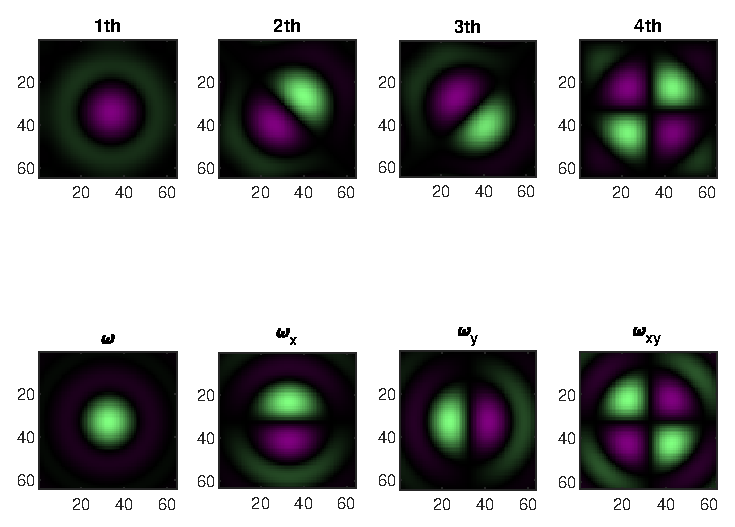
\includegraphics[width=0.9\linewidth]{../figures/gradients.eps} 
\caption{Decomposed modes} 
 \end{figure}
 
 \begin{figure}[H]
  \begin{subfigure}{.5\textwidth}
    \centering
    % include first image
    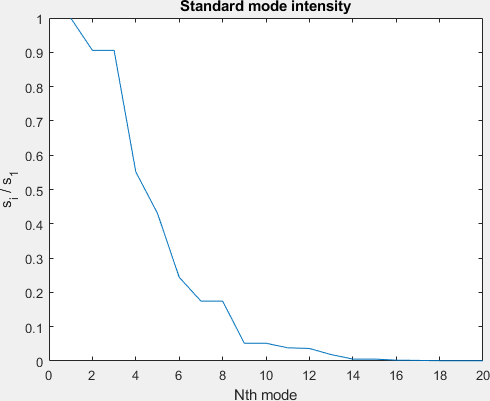
\includegraphics[width=0.9\linewidth]{../figures/singular.png}  
    %\caption{}
    \label{fig:singular}
  \end{subfigure}
  \begin{subfigure}{.5\textwidth}
    \centering
    % include second image
    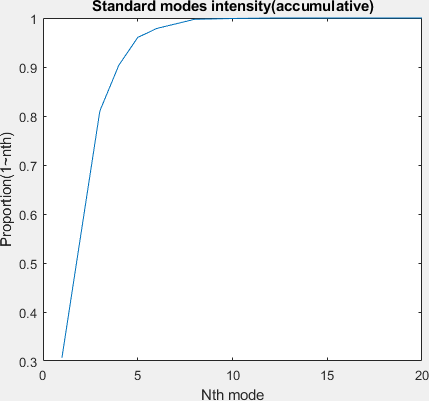
\includegraphics[width=.8\linewidth]{../figures/singular_accumative.png}  
    %\caption{Put your sub-caption here}
    \label{fig:singular_acc}
  \end{subfigure}
  \caption{The distribution of singular values of the standard density matrix $\rho$. The vertical axis in the left subfigure represents the ratio of $i^{th}$ largest singular to the first one $s_i/s_1$, and that in the right one represents $S_{cum}(i)$. The singular value decreases exponentially and the matrix is approximately low-rank. }
  \label{fig:standard singular}
  \end{figure}
  
 
  

\item Problem solving

 ADMM algorithm has been used to solve coherent Ptychography problem with convergence analysis\cite{admm}. In a partially coherent problem, an intuitive AP(alternative projection) algorithm was commonly used. We firstly extended the ADMM algorithm to mixed states, and then tried adjustments to supplement the searching process, like adding orthogonal constraints. 

We conducted simulation experiments similar to \cite{chang} and introduced performance metrics like R-factor and SNR to evaluate the reconstructed results. Our methods could overcome larger partially coherent effects compared to that in \cite{chang}, and experiment results show greater speed over AP.
 
 \begin{figure}[H]
 \centering
 \caption{}
 \begin{subfigure}{1\textwidth}
     \centering
     % include first image
     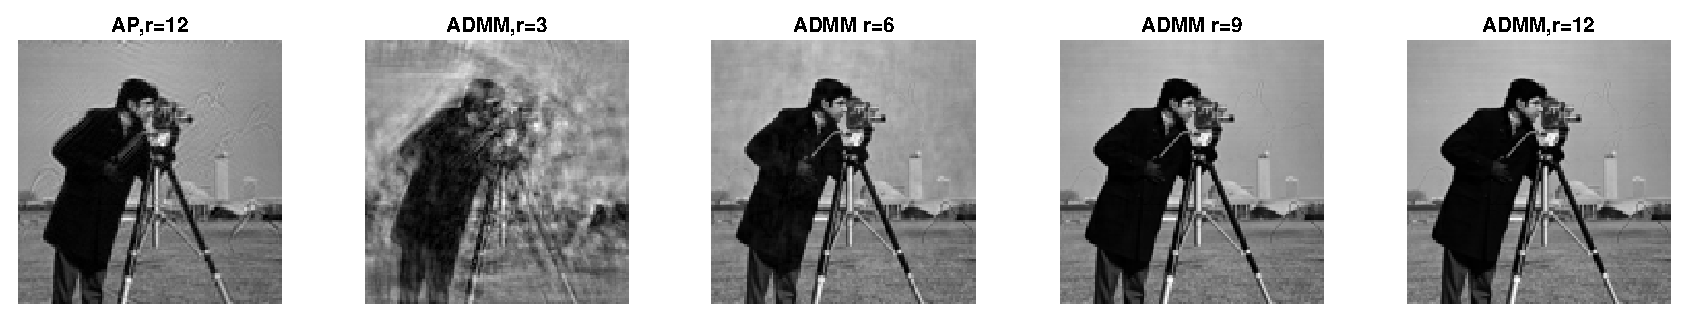
\includegraphics[width=0.9\linewidth]{../figures/modes_u.eps}  
    \caption{Amplitude}
     \label{fig:modes_u}
  \end{subfigure}
  \begin{subfigure}{1\textwidth}
     \centering
     % include second image
     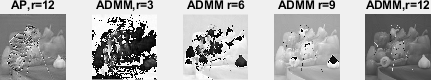
\includegraphics[width=.9\linewidth]{../figures/modes_u_phaze.png}  
     %\caption{Put your sub-caption here}
     \caption{Phase}
     \label{fig:modes_u_phaze}
  \end{subfigure}
  
     \label{fig:modes_images}
 
  \end{figure}
  
  \begin{figure}[H]
  \begin{subfigure}{.5\textwidth}
     \centering
     % include first image
     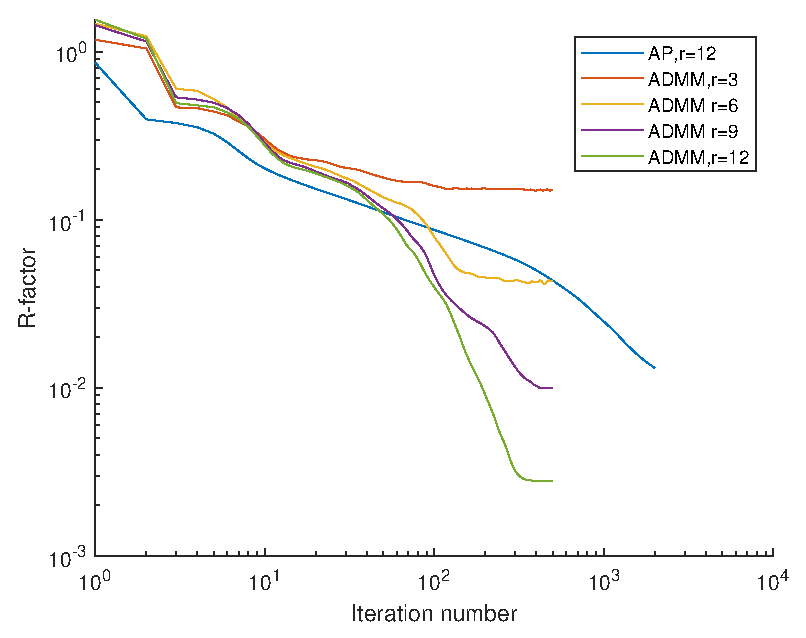
\includegraphics[width=0.9\linewidth]{../figures/modes_R.eps}  
     %\caption{}
     \label{fig:modes_R}
  \end{subfigure}
  \begin{subfigure}{.5\textwidth}
     \centering
     % include second image
     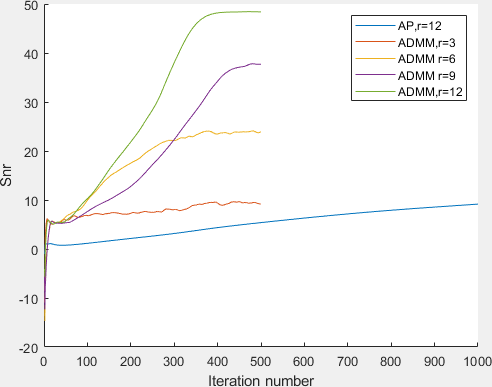
\includegraphics[width=.9\linewidth]{../figures/modes_snr.png}  
     %\caption{Put your sub-caption here}
     \label{fig:modes_snr}
  \end{subfigure}
  \caption{R and snr. }
  \label{fig:noise}
  \end{figure}



\end{enumerate}

\begin{thebibliography}{99}
\bibitem{chang}{Chang, Huibin, et al. "Partially coherent ptychography by gradient decomposition of the probe." Acta Crystallographica Section A: Foundations and Advances 74.3 (2018): 157-169.}
\bibitem{theory}{Wolf E. New theory of partial coherence in the space-frequency domain. Part I: spectra and cross spectra of steady-state sources[J]. JOSA, 1982, 72(3): 343-351.}
\bibitem{mix}{Thibault P, Menzel A. Reconstructing state mixtures from diffraction measurements[J]. Nature, 2013, 494(7435): 68-71.}
\bibitem{direct}{Tian, Lei, et al. "Multiplexed coded illumination for Fourier Ptychography with an LED array microscope." Biomedical optics express 5.7 (2014): 2376-2389.}
\bibitem{algorithm}{Thibault P, Dierolf M, Bunk O, et al. Probe retrieval in ptychographic coherent diffractive imaging[J]. Ultramicroscopy, 2009, 109(4): 338-343.}
\bibitem{quan}{Griffiths, David J., and Darrell F. Schroeter. Introduction to quantum mechanics. Cambridge University Press, 2018.}
\bibitem{all}{Fannjiang A, Strohmer T. The numerics of phase retrieval[J]. Acta Numerica, 2020, 29: 125-228.}
\bibitem{admm}{Chang, Huibin, Pablo Enfedaque, and Stefano Marchesini. "Blind ptychographic phase retrieval via convergent alternating direction method of multipliers." SIAM Journal on Imaging Sciences 12.1 (2019): 153-185.}
\bibitem{psf}{Konijnenberg S. An introduction to the theory of ptychographic phase retrieval methods[J]. Advanced Optical Technologies, 2017, 6(6): 423-438.}

\bibitem{nonconvex}{Attouch H, Bolte J, Redont P, et al. Proximal alternating minimization and projection methods for nonconvex problems: An approach based on the Kurdyka-Łojasiewicz inequality[J]. Mathematics of operations research, 2010, 35(2): 438-457.}

\bibitem{lowrank}{Candes E J, Strohmer T, Voroninski V. Phaselift: Exact and stable signal recovery from magnitude measurements via convex programming[J]. Communications on Pure and Applied Mathematics, 2013, 66(8): 1241-1274.}

\bibitem{ADMM}{Boyd S, Parikh N, Chu E. Distributed optimization and statistical learning via the alternating direction method of multipliers[M]. Now Publishers Inc, 2011.}



\end{thebibliography}




\end{document}